% Options for packages loaded elsewhere
\PassOptionsToPackage{unicode}{hyperref}
\PassOptionsToPackage{hyphens}{url}
\PassOptionsToPackage{dvipsnames,svgnames,x11names}{xcolor}
%
\documentclass[
]{book}
\title{Text Mining with R}
\usepackage{etoolbox}
\makeatletter
\providecommand{\subtitle}[1]{% add subtitle to \maketitle
  \apptocmd{\@title}{\par {\large #1 \par}}{}{}
}
\makeatother
\subtitle{A Tidy Approach}
\author{Julia Silge and David Robinson}
\date{2021-12-26}

\usepackage{amsmath,amssymb}
\usepackage{lmodern}
\usepackage{iftex}
\ifPDFTeX
  \usepackage[T1]{fontenc}
  \usepackage[utf8]{inputenc}
  \usepackage{textcomp} % provide euro and other symbols
\else % if luatex or xetex
  \usepackage{unicode-math}
  \defaultfontfeatures{Scale=MatchLowercase}
  \defaultfontfeatures[\rmfamily]{Ligatures=TeX,Scale=1}
\fi
% Use upquote if available, for straight quotes in verbatim environments
\IfFileExists{upquote.sty}{\usepackage{upquote}}{}
\IfFileExists{microtype.sty}{% use microtype if available
  \usepackage[]{microtype}
  \UseMicrotypeSet[protrusion]{basicmath} % disable protrusion for tt fonts
}{}
\makeatletter
\@ifundefined{KOMAClassName}{% if non-KOMA class
  \IfFileExists{parskip.sty}{%
    \usepackage{parskip}
  }{% else
    \setlength{\parindent}{0pt}
    \setlength{\parskip}{6pt plus 2pt minus 1pt}}
}{% if KOMA class
  \KOMAoptions{parskip=half}}
\makeatother
\usepackage{xcolor}
\IfFileExists{xurl.sty}{\usepackage{xurl}}{} % add URL line breaks if available
\IfFileExists{bookmark.sty}{\usepackage{bookmark}}{\usepackage{hyperref}}
\hypersetup{
  pdftitle={Text Mining with R},
  pdfauthor={Julia Silge and David Robinson},
  colorlinks=true,
  linkcolor={Maroon},
  filecolor={Maroon},
  citecolor={Blue},
  urlcolor={Blue},
  pdfcreator={LaTeX via pandoc}}
\urlstyle{same} % disable monospaced font for URLs
\usepackage{color}
\usepackage{fancyvrb}
\newcommand{\VerbBar}{|}
\newcommand{\VERB}{\Verb[commandchars=\\\{\}]}
\DefineVerbatimEnvironment{Highlighting}{Verbatim}{commandchars=\\\{\}}
% Add ',fontsize=\small' for more characters per line
\usepackage{framed}
\definecolor{shadecolor}{RGB}{248,248,248}
\newenvironment{Shaded}{\begin{snugshade}}{\end{snugshade}}
\newcommand{\AlertTok}[1]{\textcolor[rgb]{0.94,0.16,0.16}{#1}}
\newcommand{\AnnotationTok}[1]{\textcolor[rgb]{0.56,0.35,0.01}{\textbf{\textit{#1}}}}
\newcommand{\AttributeTok}[1]{\textcolor[rgb]{0.77,0.63,0.00}{#1}}
\newcommand{\BaseNTok}[1]{\textcolor[rgb]{0.00,0.00,0.81}{#1}}
\newcommand{\BuiltInTok}[1]{#1}
\newcommand{\CharTok}[1]{\textcolor[rgb]{0.31,0.60,0.02}{#1}}
\newcommand{\CommentTok}[1]{\textcolor[rgb]{0.56,0.35,0.01}{\textit{#1}}}
\newcommand{\CommentVarTok}[1]{\textcolor[rgb]{0.56,0.35,0.01}{\textbf{\textit{#1}}}}
\newcommand{\ConstantTok}[1]{\textcolor[rgb]{0.00,0.00,0.00}{#1}}
\newcommand{\ControlFlowTok}[1]{\textcolor[rgb]{0.13,0.29,0.53}{\textbf{#1}}}
\newcommand{\DataTypeTok}[1]{\textcolor[rgb]{0.13,0.29,0.53}{#1}}
\newcommand{\DecValTok}[1]{\textcolor[rgb]{0.00,0.00,0.81}{#1}}
\newcommand{\DocumentationTok}[1]{\textcolor[rgb]{0.56,0.35,0.01}{\textbf{\textit{#1}}}}
\newcommand{\ErrorTok}[1]{\textcolor[rgb]{0.64,0.00,0.00}{\textbf{#1}}}
\newcommand{\ExtensionTok}[1]{#1}
\newcommand{\FloatTok}[1]{\textcolor[rgb]{0.00,0.00,0.81}{#1}}
\newcommand{\FunctionTok}[1]{\textcolor[rgb]{0.00,0.00,0.00}{#1}}
\newcommand{\ImportTok}[1]{#1}
\newcommand{\InformationTok}[1]{\textcolor[rgb]{0.56,0.35,0.01}{\textbf{\textit{#1}}}}
\newcommand{\KeywordTok}[1]{\textcolor[rgb]{0.13,0.29,0.53}{\textbf{#1}}}
\newcommand{\NormalTok}[1]{#1}
\newcommand{\OperatorTok}[1]{\textcolor[rgb]{0.81,0.36,0.00}{\textbf{#1}}}
\newcommand{\OtherTok}[1]{\textcolor[rgb]{0.56,0.35,0.01}{#1}}
\newcommand{\PreprocessorTok}[1]{\textcolor[rgb]{0.56,0.35,0.01}{\textit{#1}}}
\newcommand{\RegionMarkerTok}[1]{#1}
\newcommand{\SpecialCharTok}[1]{\textcolor[rgb]{0.00,0.00,0.00}{#1}}
\newcommand{\SpecialStringTok}[1]{\textcolor[rgb]{0.31,0.60,0.02}{#1}}
\newcommand{\StringTok}[1]{\textcolor[rgb]{0.31,0.60,0.02}{#1}}
\newcommand{\VariableTok}[1]{\textcolor[rgb]{0.00,0.00,0.00}{#1}}
\newcommand{\VerbatimStringTok}[1]{\textcolor[rgb]{0.31,0.60,0.02}{#1}}
\newcommand{\WarningTok}[1]{\textcolor[rgb]{0.56,0.35,0.01}{\textbf{\textit{#1}}}}
\usepackage{longtable,booktabs,array}
\usepackage{calc} % for calculating minipage widths
% Correct order of tables after \paragraph or \subparagraph
\usepackage{etoolbox}
\makeatletter
\patchcmd\longtable{\par}{\if@noskipsec\mbox{}\fi\par}{}{}
\makeatother
% Allow footnotes in longtable head/foot
\IfFileExists{footnotehyper.sty}{\usepackage{footnotehyper}}{\usepackage{footnote}}
\makesavenoteenv{longtable}
\usepackage{graphicx}
\makeatletter
\def\maxwidth{\ifdim\Gin@nat@width>\linewidth\linewidth\else\Gin@nat@width\fi}
\def\maxheight{\ifdim\Gin@nat@height>\textheight\textheight\else\Gin@nat@height\fi}
\makeatother
% Scale images if necessary, so that they will not overflow the page
% margins by default, and it is still possible to overwrite the defaults
% using explicit options in \includegraphics[width, height, ...]{}
\setkeys{Gin}{width=\maxwidth,height=\maxheight,keepaspectratio}
% Set default figure placement to htbp
\makeatletter
\def\fps@figure{htbp}
\makeatother
% Make links footnotes instead of hotlinks:
\DeclareRobustCommand{\href}[2]{#2\footnote{\url{#1}}}
\setlength{\emergencystretch}{3em} % prevent overfull lines
\providecommand{\tightlist}{%
  \setlength{\itemsep}{0pt}\setlength{\parskip}{0pt}}
\setcounter{secnumdepth}{5}
\PassOptionsToPackage{defaults=hu-min}{magyar.ldf}
%\usepackage[utf8]{inputenc}
\usepackage[magyar]{babel}
%\usepackage{t1enc}


\usepackage{booktabs}

\newenvironment{rmdblock}[1]
  {\begin{shaded*}
  \begin{itemize}
  \renewcommand{\labelitemi}{
    \raisebox{-.7\height}[0pt][0pt]{
      {\setkeys{Gin}{width=3em,keepaspectratio}\includegraphics{images/#1}}
    }
  }
  \item
  }
  {
  \end{itemize}
  \end{shaded*}
  }
\newenvironment{rmdnote}
  {\begin{rmdblock}{note}}
  {\end{rmdblock}}
\newenvironment{rmdtip}
  {\begin{rmdblock}{tip}}
  {\end{rmdblock}}
\newenvironment{rmdwarning}
  {\begin{rmdblock}{warning}}
  {\end{rmdblock}}


\newenvironment{rmdlevel1}
  {\begin{rmdblock}{level1}}
  {\end{rmdblock}}
\newenvironment{rmdlevel2}
  {\begin{rmdblock}{level2}}
  {\end{rmdblock}}
\newenvironment{rmdlevel3}
  {\begin{rmdblock}{level3}}
  {\end{rmdblock}}
\newenvironment{rmdsummary}
  {\begin{rmdblock}{summary}}
  {\end{rmdblock}}
 \newenvironment{rmdexercise}
  {\begin{rmdblock}{exercise}}
  {\end{rmdblock}}

\ifLuaTeX
  \usepackage{selnolig}  % disable illegal ligatures
\fi
\usepackage[]{natbib}
\bibliographystyle{apalike}

\begin{document}
\maketitle

{
\hypersetup{linkcolor=}
\setcounter{tocdepth}{1}
\tableofcontents
}
\hypertarget{welcome-to-text-mining-with-r}{%
\chapter*{Welcome to Text Mining with R}\label{welcome-to-text-mining-with-r}}
\addcontentsline{toc}{chapter}{Welcome to Text Mining with R}

This is the \href{http://tidytextmining.com/}{website} for \emph{Text Mining with R}! Visit the \href{https://github.com/dgrtwo/tidy-text-mining}{GitHub repository for this site}, find the book at \href{http://www.jdoqocy.com/click-4428796-11290546?url=http\%3A\%2F\%2Fshop.oreilly.com\%2Fproduct\%2F0636920067153.do\%3Fcmp\%3Daf-strata-books-video-product_cj_0636920067153_\%25zp\&cjsku=0636920067153}{O'Reilly}, or \href{http://amzn.to/2tZkmxG}{buy it on Amazon}.

This work by \href{http://juliasilge.com/}{Julia Silge} and \href{http://varianceexplained.org/}{David Robinson} is licensed under a Creative Commons Attribution-NonCommercial-ShareAlike 3.0 United States License.

\hypertarget{preface}{%
\chapter*{Preface}\label{preface}}
\addcontentsline{toc}{chapter}{Preface}

If you work in analytics or data science, like we do, you are familiar with the fact that data is being generated all the time at ever faster rates. (You may even be a little weary of people pontificating about this fact.) Analysts are often trained to handle tabular or rectangular data that is mostly numeric, but much of the data proliferating today is unstructured and text-heavy. Many of us who work in analytical fields are not trained in even simple interpretation of natural language.

We developed the \href{https://github.com/juliasilge/tidytext}{tidytext} \citep{R-tidytext} R package because we were familiar with many methods for data wrangling and visualization, but couldn't easily apply these same methods to text. We found that using tidy data principles can make many text mining tasks easier, more effective, and consistent with tools already in wide use. Treating text as data frames of individual words allows us to manipulate, summarize, and visualize the characteristics of text easily and integrate natural language processing into effective workflows we were already using.

This book serves as an introduction of text mining using the tidytext package and other tidy tools in R. The functions provided by the tidytext package are relatively simple; what is important are the possible applications. Thus, this book provides compelling examples of real text mining problems.

\hypertarget{outline}{%
\section*{Outline}\label{outline}}
\addcontentsline{toc}{section}{Outline}

We start by introducing the tidy text format, and some of the ways dplyr, tidyr, and tidytext allow informative analyses of this structure.

\begin{itemize}
\tightlist
\item
  \textbf{Chapter \ref{tidytext}} outlines the tidy text format and the \texttt{unnest\_tokens()} function. It also introduces the gutenbergr and janeaustenr packages, which provide useful literary text datasets that we'll use throughout this book.
\item
  \textbf{Chapter \ref{sentiment}} shows how to perform sentiment analysis on a tidy text dataset, using the \texttt{sentiments} dataset from tidytext and \texttt{inner\_join()} from dplyr.
\item
  \textbf{Chapter \ref{tfidf}} describes the tf-idf statistic (term frequency times inverse document frequency), a quantity used for identifying terms that are especially important to a particular document.
\item
  \textbf{Chapter \ref{ngrams}} introduces n-grams and how to analyze word networks in text using the widyr and ggraph packages.
\end{itemize}

Text won't be tidy at all stages of an analysis, and it is important to be able to convert back and forth between tidy and non-tidy formats.

\begin{itemize}
\tightlist
\item
  \textbf{Chapter \ref{dtm}} introduces methods for tidying document-term matrices and corpus objects from the tm and quanteda packages, as well as for casting tidy text datasets into those formats.
\item
  \textbf{Chapter \ref{topicmodeling}} explores the concept of topic modeling, and uses the \texttt{tidy()} method to interpret and visualize the output of the topicmodels package.
\end{itemize}

We conclude with several case studies that bring together multiple tidy text mining approaches we've learned.

\begin{itemize}
\tightlist
\item
  \textbf{Chapter \ref{twitter}} demonstrates an application of a tidy text analysis by analyzing the authors' own Twitter archives. How do Dave's and Julia's tweeting habits compare?
\item
  \textbf{Chapter \ref{nasa}} explores metadata from over 32,000 NASA datasets (available in JSON) by looking at how keywords from the datasets are connected to title and description fields.
\item
  \textbf{Chapter \ref{usenet}} analyzes a dataset of Usenet messages from a diverse set of newsgroups (focused on topics like politics, hockey, technology, atheism, and more) to understand patterns across the groups.
\end{itemize}

\hypertarget{topics-this-book-does-not-cover}{%
\section*{Topics this book does not cover}\label{topics-this-book-does-not-cover}}
\addcontentsline{toc}{section}{Topics this book does not cover}

This book serves as an introduction to the tidy text mining framework along with a collection of examples, but it is far from a complete exploration of natural language processing. The \href{https://cran.r-project.org/web/views/NaturalLanguageProcessing.html}{CRAN Task View on Natural Language Processing} provides details on other ways to use R for computational linguistics. There are several areas that you may want to explore in more detail according to your needs.

\begin{itemize}
\tightlist
\item
  \textbf{Clustering, classification, and prediction:} Machine learning on text is a vast topic that could easily fill its own volume. We introduce one method of unsupervised clustering (topic modeling) in Chapter \ref{topicmodeling} but many more machine learning algorithms can be used in dealing with text.
\item
  \textbf{Word embedding:} One popular modern approach for text analysis is to map words to vector representations, which can then be used to examine linguistic relationships between words and to classify text. Such representations of words are not tidy in the sense that we consider here, but have found powerful applications in machine learning algorithms.
\item
  \textbf{More complex tokenization:} The tidytext package trusts the tokenizers package \citep{R-tokenizers} to perform tokenization, which itself wraps a variety of tokenizers with a consistent interface, but many others exist for specific applications.
\item
  \textbf{Languages other than English:} Some of our users have had success applying tidytext to their text mining needs for languages other than English, but we don't cover any such examples in this book.
\end{itemize}

\hypertarget{about-this-book}{%
\section*{About this book}\label{about-this-book}}
\addcontentsline{toc}{section}{About this book}

This book is focused on practical software examples and data explorations. There are few equations, but a great deal of code. We especially focus on generating real insights from the literature, news, and social media that we analyze.

We don't assume any previous knowledge of text mining. Professional linguists and text analysts will likely find our examples elementary, though we are confident they can build on the framework for their own analyses.

We do assume that the reader is at least slightly familiar with dplyr, ggplot2, and the \texttt{\%\textgreater{}\%} ``pipe'' operator in R, and is interested in applying these tools to text data. For users who don't have this background, we recommend books such as \href{http://r4ds.had.co.nz/}{R for Data Science}. We believe that with a basic background and interest in tidy data, even a user early in their R career can understand and apply our examples.

\hypertarget{using-code-examples}{%
\section*{Using code examples}\label{using-code-examples}}
\addcontentsline{toc}{section}{Using code examples}

This book was written in \href{http://www.rstudio.com/ide/}{RStudio} using \href{http://bookdown.org/}{bookdown}. The \href{https://www.tidytextmining.com/}{website} is hosted via \href{http://netlify.com/}{Netlify}, and automatically built after every push by \href{https://help.github.com/actions}{GitHub Actions}. While we show the code behind the vast majority of the analyses, in the interest of space we sometimes choose not to show the code generating a particular visualization if we've already provided the code for several similar graphs. We trust the reader can learn from and build on our examples, and the code used to generate the book can be found in our \href{https://github.com/dgrtwo/tidy-text-mining}{public GitHub repository}. We generated all plots in this book using \href{https://ggplot2.tidyverse.org/}{ggplot2} and its light theme (\texttt{theme\_light()}).

This version of the book was built with R version 4.1.2 (2021-11-01) and the following packages:

\begin{longtable}[]{@{}lll@{}}
\toprule
package & version & source \\
\midrule
\endhead
bookdown & 0.24 & CRAN (R 4.1.1) \\
dplyr & 1.0.7 & CRAN (R 4.1.1) \\
forcats & 0.5.1 & CRAN (R 4.1.0) \\
ggforce & 0.3.3 & CRAN (R 4.1.0) \\
ggplot2 & 3.3.5 & CRAN (R 4.1.1) \\
ggraph & 2.0.5 & CRAN (R 4.1.0) \\
gutenbergr & 0.2.1 & CRAN (R 4.1.0) \\
igraph & 1.2.9 & CRAN (R 4.1.2) \\
janeaustenr & 0.1.5 & CRAN (R 4.1.0) \\
jsonlite & 1.7.2 & CRAN (R 4.1.0) \\
lubridate & 1.8.0 & CRAN (R 4.1.2) \\
mallet & 1.0 & CRAN (R 4.1.0) \\
Matrix & 1.3-4 & CRAN (R 4.1.2) \\
quanteda & 3.2.0 & CRAN (R 4.1.2) \\
readr & 2.1.1 & CRAN (R 4.1.2) \\
reshape2 & 1.4.4 & CRAN (R 4.1.0) \\
sessioninfo & 1.2.1 & CRAN (R 4.1.2) \\
stringr & 1.4.0 & CRAN (R 4.1.0) \\
styler & 1.6.2 & CRAN (R 4.1.1) \\
textdata & 0.4.1 & CRAN (R 4.1.0) \\
tidyr & 1.1.4 & CRAN (R 4.1.1) \\
tidytext & 0.3.2 & CRAN (R 4.1.2) \\
tidyverse & 1.3.1 & CRAN (R 4.1.1) \\
tm & 0.7-8 & CRAN (R 4.1.0) \\
topicmodels & 0.2-12 & CRAN (R 4.1.0) \\
widyr & NA & NA \\
wordcloud & NA & NA \\
XML & 3.99-0.7 & CRAN (R 4.1.1) \\
\bottomrule
\end{longtable}

\hypertarget{tidytext}{%
\chapter{The tidy text format}\label{tidytext}}

\begin{center}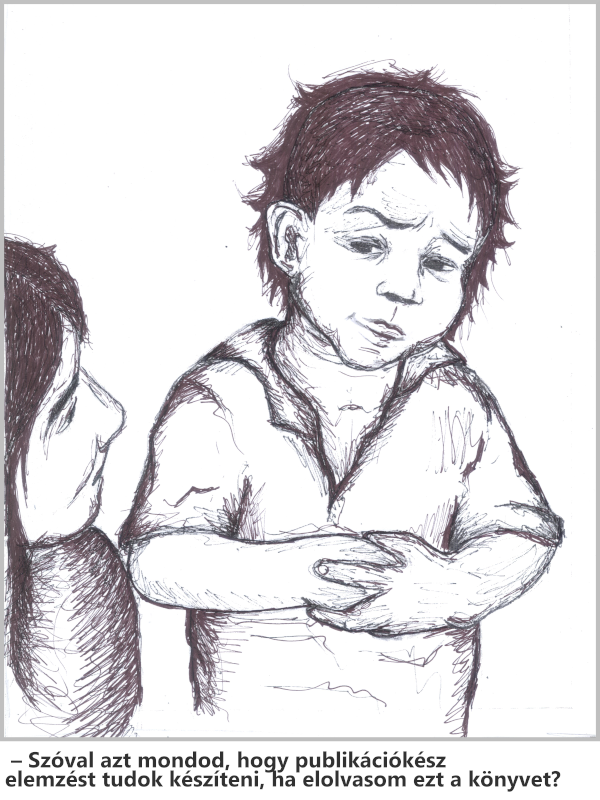
\includegraphics[width=0.9\linewidth]{images/ch_01_small} \end{center}

Using tidy data principles is a powerful way to make handling data easier and more effective, and this is no less true when it comes to dealing with text. As described by Hadley Wickham \citep{tidydata}, tidy data has a specific structure:

\begin{itemize}
\tightlist
\item
  Each variable is a column
\item
  Each observation is a row
\item
  Each type of observational unit is a table
\end{itemize}

We thus define the tidy text format as being \textbf{a table with one-token-per-row.} A token is a meaningful unit of text, such as a word, that we are interested in using for analysis, and tokenization is the process of splitting text into tokens. This one-token-per-row structure is in contrast to the ways text is often stored in current analyses, perhaps as strings or in a document-term matrix. For tidy text mining, the \textbf{token} that is stored in each row is most often a single word, but can also be an n-gram, sentence, or paragraph. In the tidytext package, we provide functionality to tokenize by commonly used units of text like these and convert to a one-term-per-row format.

Tidy data sets allow manipulation with a standard set of ``tidy'' tools, including popular packages such as dplyr \citep{R-dplyr}, tidyr \citep{R-tidyr}, ggplot2 \citep{R-ggplot2}, and broom \citep{R-broom}. By keeping the input and output in tidy tables, users can transition fluidly between these packages. We've found these tidy tools extend naturally to many text analyses and explorations.

At the same time, the tidytext package doesn't expect a user to keep text data in a tidy form at all times during an analysis. The package includes functions to \texttt{tidy()} objects (see the broom package {[}Robinson et al cited above{]}) from popular text mining R packages such as tm \citep{tm} and quanteda \citep{R-quanteda}. This allows, for example, a workflow where importing, filtering, and processing is done using dplyr and other tidy tools, after which the data is converted into a document-term matrix for machine learning applications. The models can then be re-converted into a tidy form for interpretation and visualization with ggplot2.

\hypertarget{contrasting-tidy-text-with-other-data-structures}{%
\section{Contrasting tidy text with other data structures}\label{contrasting-tidy-text-with-other-data-structures}}

As we stated above, we define the tidy text format as being a table with \textbf{one-token-per-row.} Structuring text data in this way means that it conforms to tidy data principles and can be manipulated with a set of consistent tools. This is worth contrasting with the ways text is often stored in text mining approaches.

\begin{itemize}
\tightlist
\item
  \textbf{String}: Text can, of course, be stored as strings, i.e., character vectors, within R, and often text data is first read into memory in this form.
\item
  \textbf{Corpus}: These types of objects typically contain raw strings annotated with additional metadata and details.
\item
  \textbf{Document-term matrix}: This is a sparse matrix describing a collection (i.e., a corpus) of documents with one row for each document and one column for each term. The value in the matrix is typically word count or tf-idf (see Chapter \ref{tfidf}).
\end{itemize}

Let's hold off on exploring corpus and document-term matrix objects until Chapter \ref{dtm}, and get down to the basics of converting text to a tidy format.

\hypertarget{the-unnest_tokens-function}{%
\section{\texorpdfstring{The \texttt{unnest\_tokens} function}{The unnest\_tokens function}}\label{the-unnest_tokens-function}}

Emily Dickinson wrote some lovely text in her time.

\begin{Shaded}
\begin{Highlighting}[]
\NormalTok{text }\OtherTok{\textless{}{-}} \FunctionTok{c}\NormalTok{(}\StringTok{"Because I could not stop for Death {-}"}\NormalTok{,}
          \StringTok{"He kindly stopped for me {-}"}\NormalTok{,}
          \StringTok{"The Carriage held but just Ourselves {-}"}\NormalTok{,}
          \StringTok{"and Immortality"}\NormalTok{)}

\NormalTok{text}
\CommentTok{\#\textgreater{} [1] "Because I could not stop for Death {-}"  }
\CommentTok{\#\textgreater{} [2] "He kindly stopped for me {-}"            }
\CommentTok{\#\textgreater{} [3] "The Carriage held but just Ourselves {-}"}
\CommentTok{\#\textgreater{} [4] "and Immortality"}
\end{Highlighting}
\end{Shaded}

This is a typical character vector that we might want to analyze. In order to turn it into a tidy text dataset, we first need to put it into a data frame.

\begin{Shaded}
\begin{Highlighting}[]
\FunctionTok{library}\NormalTok{(dplyr)}
\NormalTok{text\_df }\OtherTok{\textless{}{-}} \FunctionTok{tibble}\NormalTok{(}\AttributeTok{line =} \DecValTok{1}\SpecialCharTok{:}\DecValTok{4}\NormalTok{, }\AttributeTok{text =}\NormalTok{ text)}

\NormalTok{text\_df}
\CommentTok{\#\textgreater{} \# A tibble: 4 x 2}
\CommentTok{\#\textgreater{}    line text                                  }
\CommentTok{\#\textgreater{}   \textless{}int\textgreater{} \textless{}chr\textgreater{}                                 }
\CommentTok{\#\textgreater{} 1     1 Because I could not stop for Death {-}  }
\CommentTok{\#\textgreater{} 2     2 He kindly stopped for me {-}            }
\CommentTok{\#\textgreater{} 3     3 The Carriage held but just Ourselves {-}}
\CommentTok{\#\textgreater{} 4     4 and Immortality}
\end{Highlighting}
\end{Shaded}

What does it mean that this data frame has printed out as a ``tibble''? A tibble is a modern class of data frame within R, available in the dplyr and tibble packages, that has a convenient print method, will not convert strings to factors, and does not use row names. Tibbles are great for use with tidy tools.

Notice that this data frame containing text isn't yet compatible with tidy text analysis, though. We can't filter out words or count which occur most frequently, since each row is made up of multiple combined words. We need to convert this so that it has \textbf{one-token-per-document-per-row}.

\begin{rmdexercise}
A token is a meaningful unit of text, most often a word, that we are
interested in using for further analysis, and tokenization is the
process of splitting text into tokens.
\end{rmdexercise}

In this first example, we only have one document (the poem), but we will explore examples with multiple documents soon.

Within our tidy text framework, we need to both break the text into individual tokens (a process called \emph{tokenization}) \emph{and} transform it to a tidy data structure. To do this, we use tidytext's \texttt{unnest\_tokens()} function.

\begin{Shaded}
\begin{Highlighting}[]
\FunctionTok{library}\NormalTok{(tidytext)}

\NormalTok{text\_df }\SpecialCharTok{\%\textgreater{}\%}
  \FunctionTok{unnest\_tokens}\NormalTok{(word, text)}
\CommentTok{\#\textgreater{} \# A tibble: 20 x 2}
\CommentTok{\#\textgreater{}     line word   }
\CommentTok{\#\textgreater{}    \textless{}int\textgreater{} \textless{}chr\textgreater{}  }
\CommentTok{\#\textgreater{}  1     1 because}
\CommentTok{\#\textgreater{}  2     1 i      }
\CommentTok{\#\textgreater{}  3     1 could  }
\CommentTok{\#\textgreater{}  4     1 not    }
\CommentTok{\#\textgreater{}  5     1 stop   }
\CommentTok{\#\textgreater{}  6     1 for    }
\CommentTok{\#\textgreater{}  7     1 death  }
\CommentTok{\#\textgreater{}  8     2 he     }
\CommentTok{\#\textgreater{}  9     2 kindly }
\CommentTok{\#\textgreater{} 10     2 stopped}
\CommentTok{\#\textgreater{} \# ... with 10 more rows}
\end{Highlighting}
\end{Shaded}

The two basic arguments to \texttt{unnest\_tokens} used here are column names. First we have the output column name that will be created as the text is unnested into it (\texttt{word}, in this case), and then the input column that the text comes from (\texttt{text}, in this case). Remember that \texttt{text\_df} above has a column called \texttt{text} that contains the data of interest.

After using \texttt{unnest\_tokens}, we've split each row so that there is one token (word) in each row of the new data frame; the default tokenization in \texttt{unnest\_tokens()} is for single words, as shown here. Also notice:

\begin{itemize}
\tightlist
\item
  Other columns, such as the line number each word came from, are retained.
\item
  Punctuation has been stripped.
\item
  By default, \texttt{unnest\_tokens()} converts the tokens to lowercase, which makes them easier to compare or combine with other datasets. (Use the \texttt{to\_lower\ =\ FALSE} argument to turn off this behavior).
\end{itemize}

Having the text data in this format lets us manipulate, process, and visualize the text using the standard set of tidy tools, namely dplyr, tidyr, and ggplot2, as shown in Figure \ref{fig:tidyflow-ch1}.

\hypertarget{tidyausten}{%
\section{Tidying the works of Jane Austen}\label{tidyausten}}

Let's use the text of Jane Austen's 6 completed, published novels from the \href{https://cran.r-project.org/package=janeaustenr}{janeaustenr} package \citep{R-janeaustenr}, and transform them into a tidy format. The janeaustenr package provides these texts in a one-row-per-line format, where a line in this context is analogous to a literal printed line in a physical book. Let's start with that, and also use \texttt{mutate()} to annotate a \texttt{linenumber} quantity to keep track of lines in the original format and a \texttt{chapter} (using a regex) to find where all the chapters are.

\begin{Shaded}
\begin{Highlighting}[]
\FunctionTok{library}\NormalTok{(janeaustenr)}
\FunctionTok{library}\NormalTok{(dplyr)}
\FunctionTok{library}\NormalTok{(stringr)}

\NormalTok{original\_books }\OtherTok{\textless{}{-}} \FunctionTok{austen\_books}\NormalTok{() }\SpecialCharTok{\%\textgreater{}\%}
  \FunctionTok{group\_by}\NormalTok{(book) }\SpecialCharTok{\%\textgreater{}\%}
  \FunctionTok{mutate}\NormalTok{(}\AttributeTok{linenumber =} \FunctionTok{row\_number}\NormalTok{(),}
         \AttributeTok{chapter =} \FunctionTok{cumsum}\NormalTok{(}\FunctionTok{str\_detect}\NormalTok{(text, }
                                     \FunctionTok{regex}\NormalTok{(}\StringTok{"\^{}chapter [}\SpecialCharTok{\textbackslash{}\textbackslash{}}\StringTok{divxlc]"}\NormalTok{,}
                                           \AttributeTok{ignore\_case =} \ConstantTok{TRUE}\NormalTok{)))) }\SpecialCharTok{\%\textgreater{}\%}
  \FunctionTok{ungroup}\NormalTok{()}

\NormalTok{original\_books}
\CommentTok{\#\textgreater{} \# A tibble: 73,422 x 4}
\CommentTok{\#\textgreater{}    text                    book                linenumber chapter}
\CommentTok{\#\textgreater{}    \textless{}chr\textgreater{}                   \textless{}fct\textgreater{}                    \textless{}int\textgreater{}   \textless{}int\textgreater{}}
\CommentTok{\#\textgreater{}  1 "SENSE AND SENSIBILITY" Sense \& Sensibility          1       0}
\CommentTok{\#\textgreater{}  2 ""                      Sense \& Sensibility          2       0}
\CommentTok{\#\textgreater{}  3 "by Jane Austen"        Sense \& Sensibility          3       0}
\CommentTok{\#\textgreater{}  4 ""                      Sense \& Sensibility          4       0}
\CommentTok{\#\textgreater{}  5 "(1811)"                Sense \& Sensibility          5       0}
\CommentTok{\#\textgreater{}  6 ""                      Sense \& Sensibility          6       0}
\CommentTok{\#\textgreater{}  7 ""                      Sense \& Sensibility          7       0}
\CommentTok{\#\textgreater{}  8 ""                      Sense \& Sensibility          8       0}
\CommentTok{\#\textgreater{}  9 ""                      Sense \& Sensibility          9       0}
\CommentTok{\#\textgreater{} 10 "CHAPTER 1"             Sense \& Sensibility         10       1}
\CommentTok{\#\textgreater{} \# ... with 73,412 more rows}
\end{Highlighting}
\end{Shaded}

To work with this as a tidy dataset, we need to restructure it in the \textbf{one-token-per-row} format, which as we saw earlier is done with the \texttt{unnest\_tokens()} function.

\begin{Shaded}
\begin{Highlighting}[]
\FunctionTok{library}\NormalTok{(tidytext)}
\NormalTok{tidy\_books }\OtherTok{\textless{}{-}}\NormalTok{ original\_books }\SpecialCharTok{\%\textgreater{}\%}
  \FunctionTok{unnest\_tokens}\NormalTok{(word, text)}

\NormalTok{tidy\_books}
\CommentTok{\#\textgreater{} \# A tibble: 725,055 x 4}
\CommentTok{\#\textgreater{}    book                linenumber chapter word       }
\CommentTok{\#\textgreater{}    \textless{}fct\textgreater{}                    \textless{}int\textgreater{}   \textless{}int\textgreater{} \textless{}chr\textgreater{}      }
\CommentTok{\#\textgreater{}  1 Sense \& Sensibility          1       0 sense      }
\CommentTok{\#\textgreater{}  2 Sense \& Sensibility          1       0 and        }
\CommentTok{\#\textgreater{}  3 Sense \& Sensibility          1       0 sensibility}
\CommentTok{\#\textgreater{}  4 Sense \& Sensibility          3       0 by         }
\CommentTok{\#\textgreater{}  5 Sense \& Sensibility          3       0 jane       }
\CommentTok{\#\textgreater{}  6 Sense \& Sensibility          3       0 austen     }
\CommentTok{\#\textgreater{}  7 Sense \& Sensibility          5       0 1811       }
\CommentTok{\#\textgreater{}  8 Sense \& Sensibility         10       1 chapter    }
\CommentTok{\#\textgreater{}  9 Sense \& Sensibility         10       1 1          }
\CommentTok{\#\textgreater{} 10 Sense \& Sensibility         13       1 the        }
\CommentTok{\#\textgreater{} \# ... with 725,045 more rows}
\end{Highlighting}
\end{Shaded}

This function uses the \href{https://github.com/ropensci/tokenizers}{tokenizers} package to separate each line of text in the original data frame into tokens. The default tokenizing is for words, but other options include characters, n-grams, sentences, lines, paragraphs, or separation around a regex pattern.

Now that the data is in one-word-per-row format, we can manipulate it with tidy tools like dplyr. Often in text analysis, we will want to remove stop words; stop words are words that are not useful for an analysis, typically extremely common words such as ``the'', ``of'', ``to'', and so forth in English. We can remove stop words (kept in the tidytext dataset \texttt{stop\_words}) with an \texttt{anti\_join()}.

\begin{Shaded}
\begin{Highlighting}[]
\FunctionTok{data}\NormalTok{(stop\_words)}

\NormalTok{tidy\_books }\OtherTok{\textless{}{-}}\NormalTok{ tidy\_books }\SpecialCharTok{\%\textgreater{}\%}
  \FunctionTok{anti\_join}\NormalTok{(stop\_words)}
\end{Highlighting}
\end{Shaded}

The \texttt{stop\_words} dataset in the tidytext package contains stop words from three lexicons. We can use them all together, as we have here, or \texttt{filter()} to only use one set of stop words if that is more appropriate for a certain analysis.

We can also use dplyr's \texttt{count()} to find the most common words in all the books as a whole.

\begin{Shaded}
\begin{Highlighting}[]
\NormalTok{tidy\_books }\SpecialCharTok{\%\textgreater{}\%}
  \FunctionTok{count}\NormalTok{(word, }\AttributeTok{sort =} \ConstantTok{TRUE}\NormalTok{) }
\CommentTok{\#\textgreater{} \# A tibble: 13,914 x 2}
\CommentTok{\#\textgreater{}    word       n}
\CommentTok{\#\textgreater{}    \textless{}chr\textgreater{}  \textless{}int\textgreater{}}
\CommentTok{\#\textgreater{}  1 miss    1855}
\CommentTok{\#\textgreater{}  2 time    1337}
\CommentTok{\#\textgreater{}  3 fanny    862}
\CommentTok{\#\textgreater{}  4 dear     822}
\CommentTok{\#\textgreater{}  5 lady     817}
\CommentTok{\#\textgreater{}  6 sir      806}
\CommentTok{\#\textgreater{}  7 day      797}
\CommentTok{\#\textgreater{}  8 emma     787}
\CommentTok{\#\textgreater{}  9 sister   727}
\CommentTok{\#\textgreater{} 10 house    699}
\CommentTok{\#\textgreater{} \# ... with 13,904 more rows}
\end{Highlighting}
\end{Shaded}

Because we've been using tidy tools, our word counts are stored in a tidy data frame. This allows us to pipe this directly to the ggplot2 package, for example to create a visualization of the most common words (Figure \ref{fig:plotcount}).

\begin{Shaded}
\begin{Highlighting}[]
\FunctionTok{library}\NormalTok{(ggplot2)}

\NormalTok{tidy\_books }\SpecialCharTok{\%\textgreater{}\%}
  \FunctionTok{count}\NormalTok{(word, }\AttributeTok{sort =} \ConstantTok{TRUE}\NormalTok{) }\SpecialCharTok{\%\textgreater{}\%}
  \FunctionTok{filter}\NormalTok{(n }\SpecialCharTok{\textgreater{}} \DecValTok{600}\NormalTok{) }\SpecialCharTok{\%\textgreater{}\%}
  \FunctionTok{mutate}\NormalTok{(}\AttributeTok{word =} \FunctionTok{reorder}\NormalTok{(word, n)) }\SpecialCharTok{\%\textgreater{}\%}
  \FunctionTok{ggplot}\NormalTok{(}\FunctionTok{aes}\NormalTok{(n, word)) }\SpecialCharTok{+}
  \FunctionTok{geom\_col}\NormalTok{() }\SpecialCharTok{+}
  \FunctionTok{labs}\NormalTok{(}\AttributeTok{y =} \ConstantTok{NULL}\NormalTok{)}
\end{Highlighting}
\end{Shaded}

\begin{figure}

{\centering 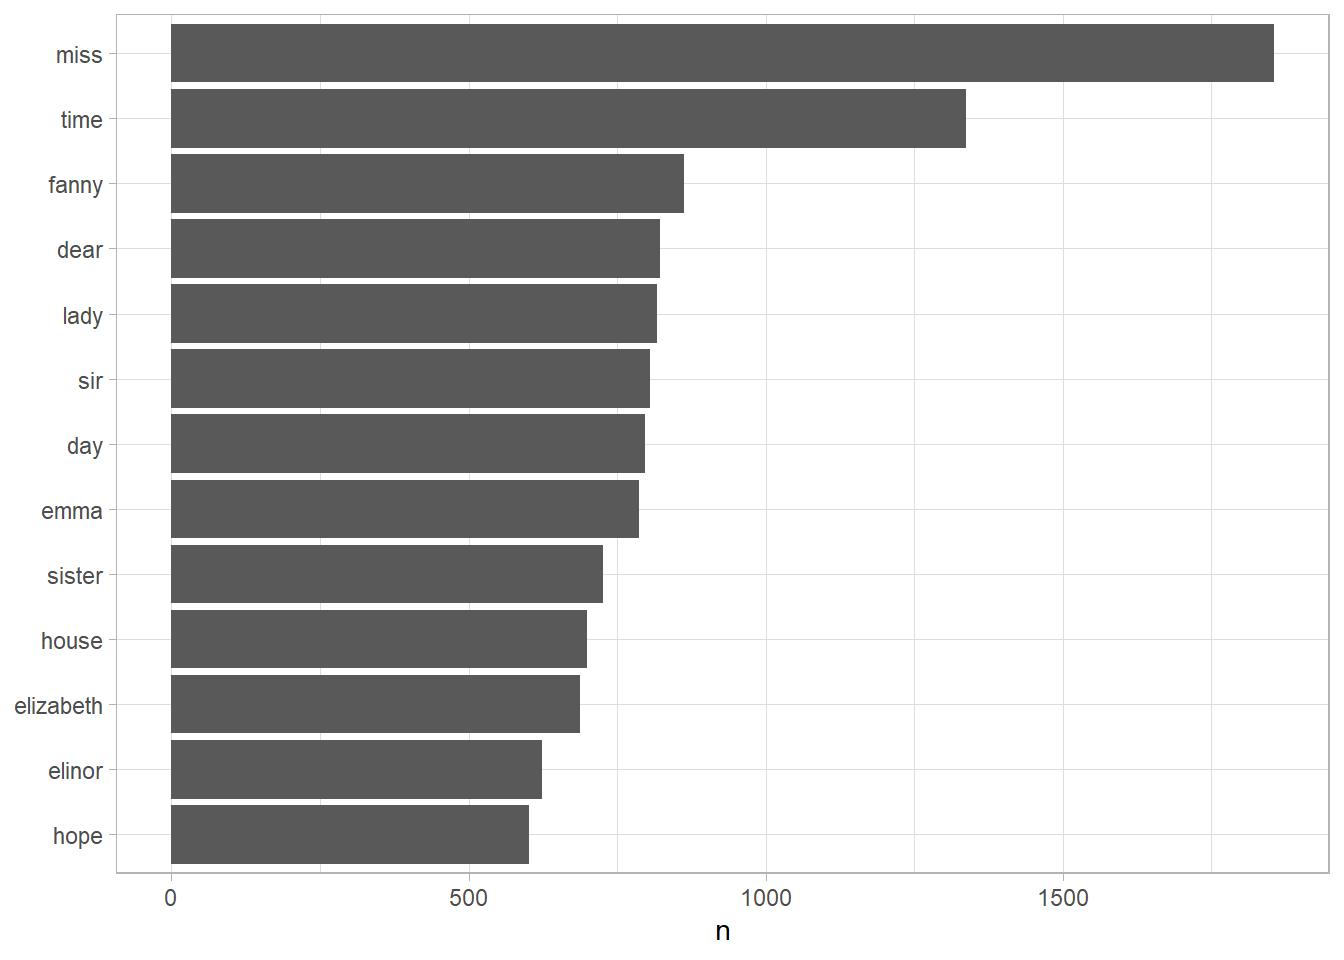
\includegraphics[width=0.9\linewidth]{01-tidy-text_files/figure-latex/plotcount-1} 

}

\caption{The most common words in Jane Austen's novels}\label{fig:plotcount}
\end{figure}

Note that the \texttt{austen\_books()} function started us with exactly the text we wanted to analyze, but in other cases we may need to perform cleaning of text data, such as removing copyright headers or formatting. You'll see examples of this kind of pre-processing in the case study chapters, particularly Chapter \ref{pre-processing-text}.

\hypertarget{the-gutenbergr-package}{%
\section{The gutenbergr package}\label{the-gutenbergr-package}}

Now that we've used the janeaustenr package to explore tidying text, let's introduce the \href{https://github.com/ropensci/gutenbergr}{gutenbergr} package \citep{R-gutenbergr}. The gutenbergr package provides access to the public domain works from the \href{https://www.gutenberg.org/}{Project Gutenberg} collection. The package includes tools both for downloading books (stripping out the unhelpful header/footer information), and a complete dataset of Project Gutenberg metadata that can be used to find works of interest. In this book, we will mostly use the function \texttt{gutenberg\_download()} that downloads one or more works from Project Gutenberg by ID, but you can also use other functions to explore metadata, pair Gutenberg ID with title, author, language, etc., or gather information about authors.

\begin{rmdlevel1}
\textbf{Szint 1}

\begin{itemize}
\tightlist
\item
  kjdshfksdhjksdhf
\item
  sdfaj \texttt{adqweqweqwe} akjlkjf
\end{itemize}

To learn more about gutenbergr, check out the
\href{https://docs.ropensci.org/gutenbergr/}{package's documentation at
rOpenSci}, where it is one of rOpenSci's packages for data access.
\end{rmdlevel1}

\begin{rmdlevel2}
To learn more about gutenbergr, check out the
\href{https://docs.ropensci.org/gutenbergr/}{package's documentation at
rOpenSci}, where it is one of rOpenSci's packages for data access.
\end{rmdlevel2}

\begin{rmdlevel3}
To learn more about gutenbergr, check out the
\href{https://docs.ropensci.org/gutenbergr/}{package's documentation at
rOpenSci}, where it is one of rOpenSci's packages for data access.
\end{rmdlevel3}

\begin{rmdsummary}
To learn more about gutenbergr, check out the
\href{https://docs.ropensci.org/gutenbergr/}{package's documentation at
rOpenSci}, where it is one of rOpenSci's packages for data access.
\end{rmdsummary}

\begin{rmdexercise}
To learn more about gutenbergr, check out the
\href{https://docs.ropensci.org/gutenbergr/}{package's documentation at
rOpenSci}, where it is one of rOpenSci's packages for data access.
\end{rmdexercise}

\hypertarget{word-frequencies}{%
\section{Word frequencies}\label{word-frequencies}}

A common task in text mining is to look at word frequencies, just like we have done above for Jane Austen's novels, and to compare frequencies across different texts. We can do this intuitively and smoothly using tidy data principles. We already have Jane Austen's works; let's get two more sets of texts to compare to. First, let's look at some science fiction and fantasy novels by H.G. Wells, who lived in the late 19th and early 20th centuries. Let's get \href{https://www.gutenberg.org/ebooks/35}{\emph{The Time Machine}}, \href{https://www.gutenberg.org/ebooks/36}{\emph{The War of the Worlds}}, \href{https://www.gutenberg.org/ebooks/5230}{\emph{The Invisible Man}}, and \href{https://www.gutenberg.org/ebooks/159}{\emph{The Island of Doctor Moreau}}. We can access these works using \texttt{gutenberg\_download()} and the Project Gutenberg ID numbers for each novel.

\begin{Shaded}
\begin{Highlighting}[]
\FunctionTok{library}\NormalTok{(gutenbergr)}

\NormalTok{hgwells }\OtherTok{\textless{}{-}} \FunctionTok{gutenberg\_download}\NormalTok{(}\FunctionTok{c}\NormalTok{(}\DecValTok{35}\NormalTok{, }\DecValTok{36}\NormalTok{, }\DecValTok{5230}\NormalTok{, }\DecValTok{159}\NormalTok{))}
\end{Highlighting}
\end{Shaded}

\hypertarget{summary}{%
\section{Summary}\label{summary}}

In this chapter, we explored what we mean by tidy data when it comes to text, and how tidy data principles can be applied to natural language processing. When text is organized in a format with one token per row, tasks like removing stop words or calculating word frequencies are natural applications of familiar operations within the tidy tool ecosystem. The one-token-per-row framework can be extended from single words to n-grams and other meaningful units of text, as well as to many other analysis priorities that we will consider in this book.

\hypertarget{tidynntext}{%
\chapter{Thidy text format}\label{tidynntext}}

\begin{center}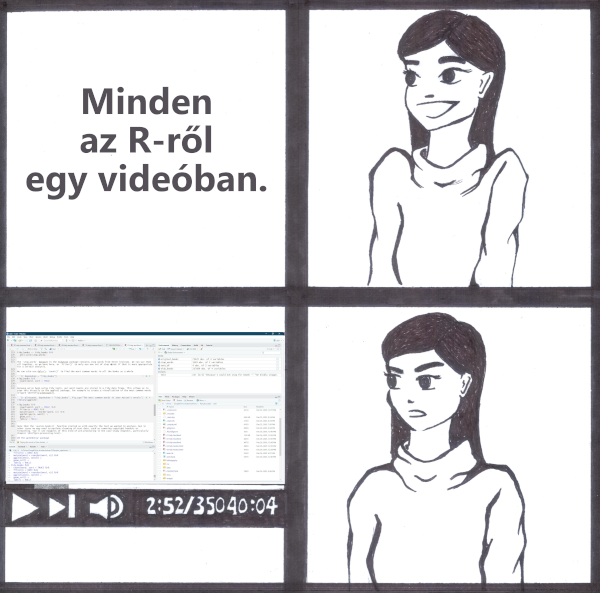
\includegraphics[width=0.9\linewidth]{images/ch_02_small} \end{center}

Using tidy data principles is a powerful way to make handling data easier and more effective, and this is no less true when it comes to dealing with text. As described by Hadley Wickham \citep{tidydata}, tidy data has a specific structure:

\begin{itemize}
\tightlist
\item
  Each variable is a column
\item
  Each observation is a row
\item
  Each type of observational unit is a table
\end{itemize}

\hypertarget{tidynnddddtext}{%
\chapter{Thidy text format}\label{tidynnddddtext}}

\begin{center}
\includegraphics[width=0.9\linewidth]{images/ch_03_small} \end{center}

Using tidy data principles is a powerful way to make handling data easier and more effective, and this is no less true when it comes to dealing with text. As described by Hadley Wickham \citep{tidydata}, tidy data has a specific structure:

\begin{itemize}
\tightlist
\item
  Each variable is a column
\item
  Each observation is a row
\item
  Each type of observational unit is a table
\end{itemize}

\hypertarget{tidynnddddtqqqext}{%
\chapter{Thidy text format}\label{tidynnddddtqqqext}}

\begin{center}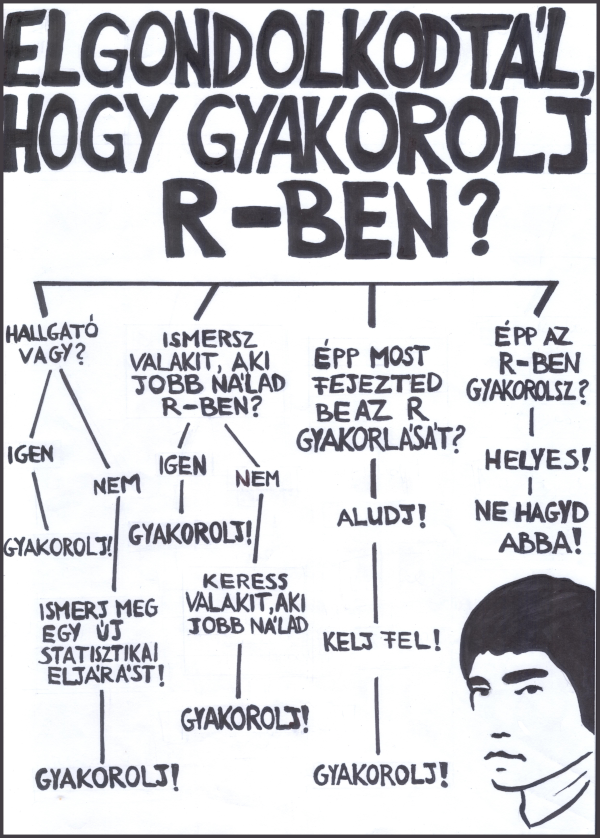
\includegraphics[width=0.9\linewidth]{images/ch_04_small} \end{center}

Using tidy data principles is a powerful way to make handling data easier and more effective, and this is no less true when it comes to dealing with text. As described by Hadley Wickham \citep{tidydata}, tidy data has a specific structure:

\begin{itemize}
\tightlist
\item
  Each variable is a column
\item
  Each observation is a row
\item
  Each type of observational unit is a table
\end{itemize}

\hypertarget{thijhhdy-text-formatnnn}{%
\chapter{Thijhhdy text formatnnn}\label{thijhhdy-text-formatnnn}}

\begin{center}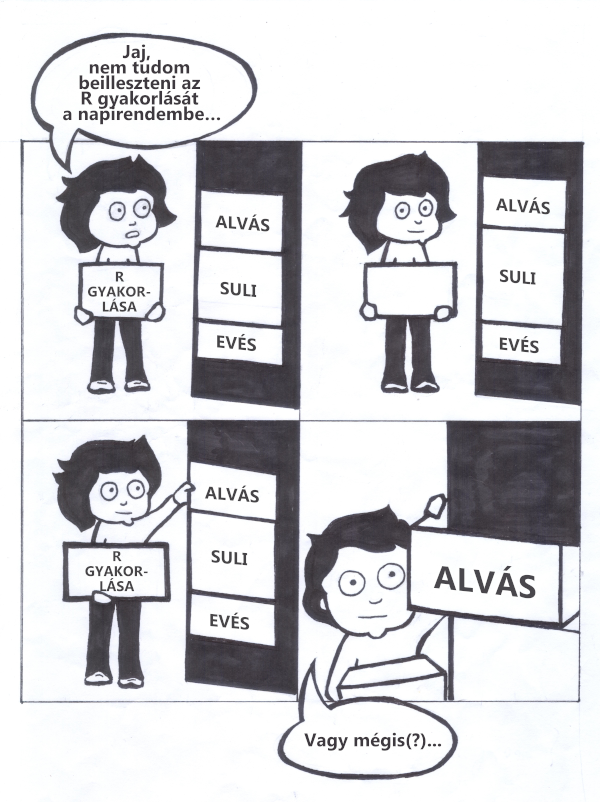
\includegraphics[width=0.9\linewidth]{images/ch_05_small} \end{center}

Using tidy data principles is a powerful way to make handling data easier and more effective, and this is no less true when it comes to dealing with text. As described by Hadley Wickham \citep{tidydata}, tidy data has a specific structure:

\begin{itemize}
\tightlist
\item
  Each variable is a column
\item
  Each observation is a row
\item
  Each type of observational unit is a table
\end{itemize}

\hypertarget{thijaahdy-text-formatnnnsss}{%
\chapter{Thijaahdy text formatnnnsss}\label{thijaahdy-text-formatnnnsss}}

\begin{center}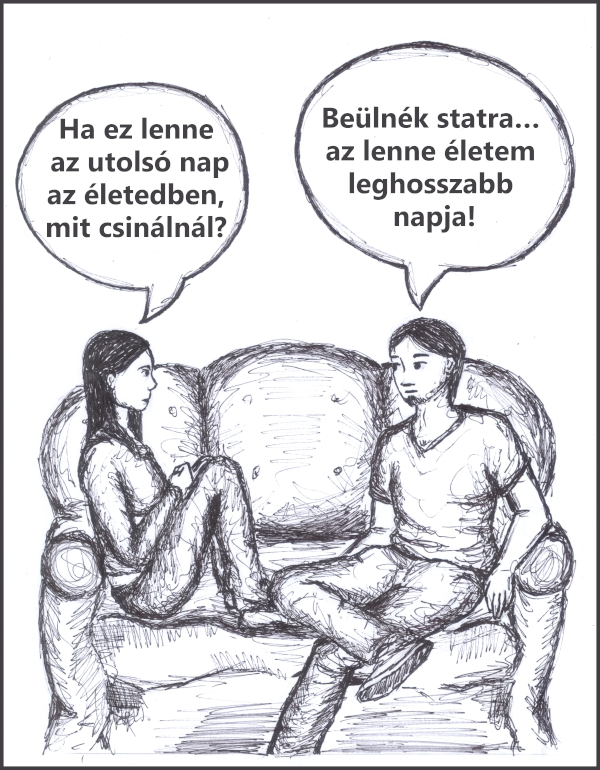
\includegraphics[width=0.9\linewidth]{images/ch_06_small} \end{center}

Using tidy data principles is a powerful way to make handling data easier and more effective, and this is no less true when it comes to dealing with text. As described by Hadley Wickham \citep{tidydata}, tidy data has a specific structure:

\begin{itemize}
\tightlist
\item
  Each variable is a column
\item
  Each observation is a row
\item
  Each type of observational unit is a table
\end{itemize}

\hypertarget{thijaashdy-text-formatnnnsss}{%
\chapter{Thijaashdy text formatnnnsss}\label{thijaashdy-text-formatnnnsss}}

\begin{center}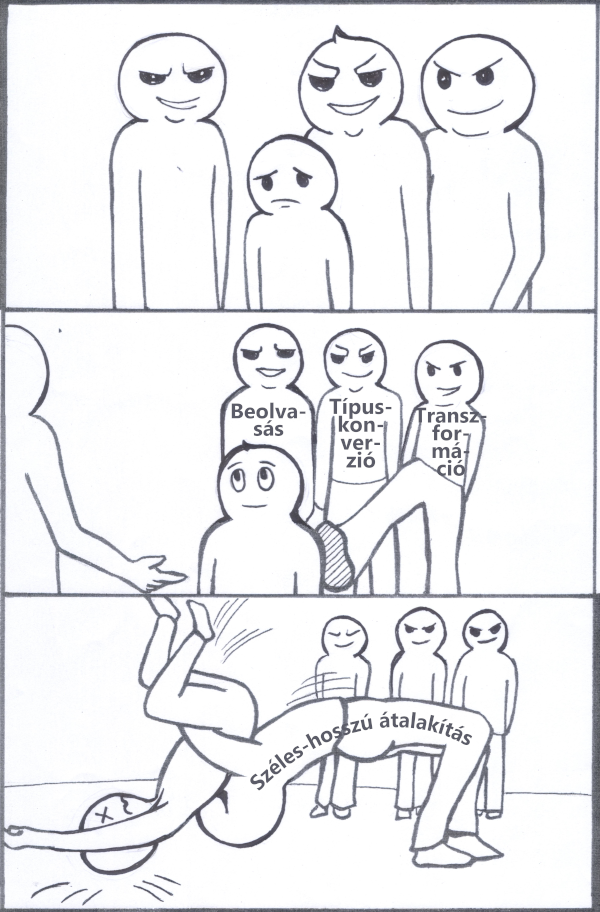
\includegraphics[width=0.9\linewidth]{images/ch_07_small} \end{center}

Using tidy data principles is a powerful way to make handling data easier and more effective, and this is no less true when it comes to dealing with text. As described by Hadley Wickham \citep{tidydata}, tidy data has a specific structure:

\begin{itemize}
\tightlist
\item
  Each variable is a column
\item
  Each observation is a row
\item
  Each type of observational unit is a table
\end{itemize}

\hypertarget{thijaashdsdfsy-text-formatnnnsss}{%
\chapter{Thijaashdsdfsy text formatnnnsss}\label{thijaashdsdfsy-text-formatnnnsss}}

\begin{center}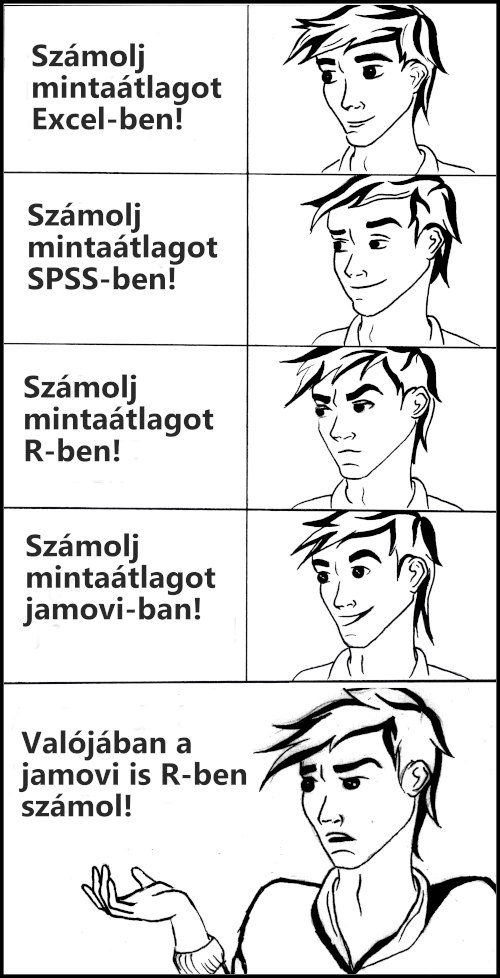
\includegraphics[width=0.9\linewidth]{images/ch_08_small} \end{center}

Using tidy data principles is a powerful way to make handling data easier and more effective, and this is no less true when it comes to dealing with text. As described by Hadley Wickham \citep{tidydata}, tidy data has a specific structure:

\begin{itemize}
\tightlist
\item
  Each variable is a column
\item
  Each observation is a row
\item
  Each type of observational unit is a table
\end{itemize}

\hypertarget{thijaashdsdfsy-text-formatnnnsss-1}{%
\chapter{Thijaashdsdfsy text formatnnnsss}\label{thijaashdsdfsy-text-formatnnnsss-1}}

\begin{center}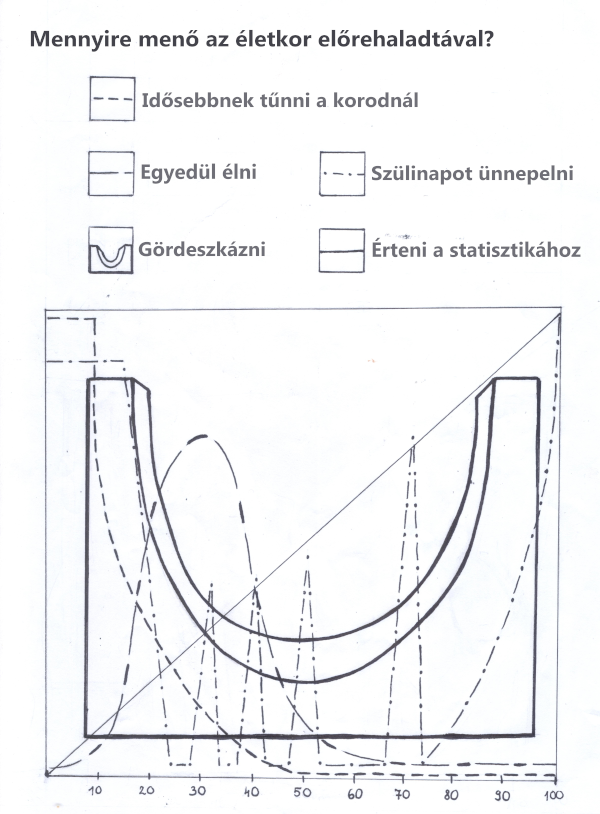
\includegraphics[width=0.9\linewidth]{images/ch_09_small} \end{center}

Using tidy data principles is a powerful way to make handling data easier and more effective, and this is no less true when it comes to dealing with text. As described by Hadley Wickham \citep{tidydata}, tidy data has a specific structure:

\begin{itemize}
\tightlist
\item
  Each variable is a column
\item
  Each observation is a row
\item
  Each type of observational unit is a table
\end{itemize}

\hypertarget{thijaashdsdfsys-text-formatnnnsss}{%
\chapter{Thijaashdsdfsys text formatnnnsss}\label{thijaashdsdfsys-text-formatnnnsss}}

\begin{center}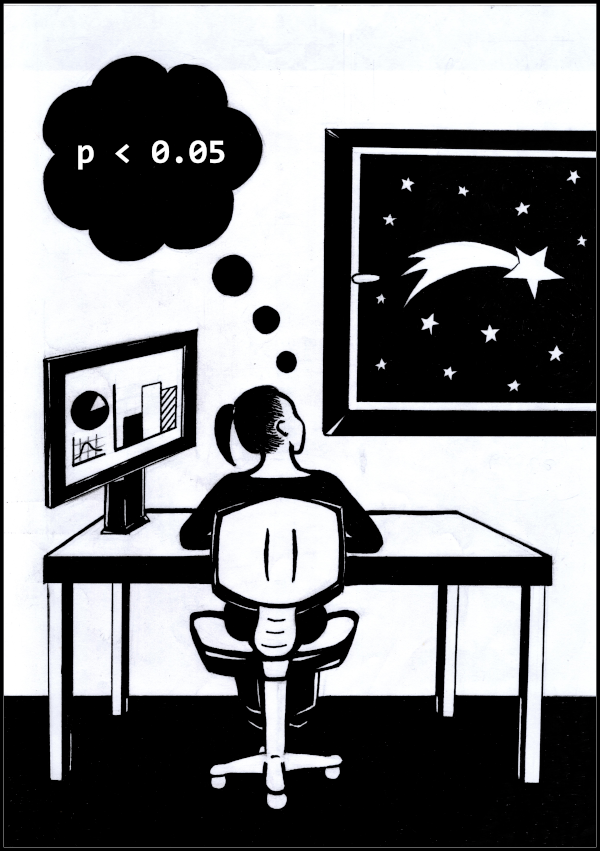
\includegraphics[width=0.9\linewidth]{images/ch_10_small} \end{center}

Using tidy data principles is a powerful way to make handling data easier and more effective, and this is no less true when it comes to dealing with text. As described by Hadley Wickham \citep{tidydata}, tidy data has a specific structure:

\begin{itemize}
\tightlist
\item
  Each variable is a column
\item
  Each observation is a row
\item
  Each type of observational unit is a table
\end{itemize}

\hypertarget{thijaashdswdfsys-text-formatnnnsss}{%
\chapter{Thijaashdswdfsys text formatnnnsss}\label{thijaashdswdfsys-text-formatnnnsss}}

\begin{center}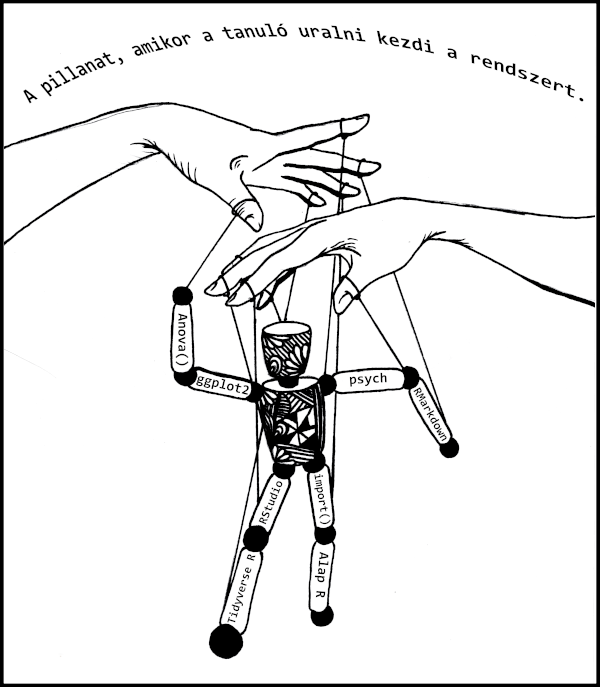
\includegraphics[width=0.9\linewidth]{images/ch_11_small} \end{center}

Using tidy data principles is a powerful way to make handling data easier and more effective, and this is no less true when it comes to dealing with text. As described by Hadley Wickham \citep{tidydata}, tidy data has a specific structure:

\begin{itemize}
\tightlist
\item
  Each variable is a column
\item
  Each observation is a row
\item
  Each type of observational unit is a table
\end{itemize}

\end{document}
